\documentclass{article}
\title{The Ant Colony Optimisation for the Travelling Salesman Problem}
\author{Dylan Galea}

\usepackage{cite}
\usepackage{amsmath}
\usepackage{amsthm}
\usepackage{amssymb}
\usepackage{physics}
\usepackage{tikz}
\usetikzlibrary{arrows.meta,automata,positioning}

\newtheorem{definition}{Definition}[subsection]
\newtheorem{theorem}[definition]{Theorem}
\newtheorem{lemma}[definition]{Lemma}
\newtheorem*{remark}{Remark}
\newtheorem{example}[definition]{Example}

\begin{document}
\maketitle
\newpage
\tableofcontents
\newpage
\section{Introduction}
Before defining the Travelling Salesman Problem and proving properties about it, a number of graph theoretic concepts that will be used throughout, must first be defined. Therefore, what follows is a sub-section that introduces a number of graph theoretic concepts which are required for the Travelling Salesman Problem.
\subsection{Some Graph Theory}
Graph theory is the study of a structure called a graph. A graph can be defined formally as shown in definition \ref{Graph} below.
\begin{definition}
\label{Graph}
A graph G is a pair (V,E) were V is any non empty finite set called the set of vertices of G, and E $\subseteq$ \{$\{u,v\}$ $:$ $\forall$ u,v $\in$ V and u $\neq$ v\} is called the set of edges of G {\normalfont{\cite{black_tanenbaum_2017}}}. A graph G defined by the pair (V,E) is denoted by G(V,E) or G.
\end{definition}
A graph defined using definition \ref{Graph} is called an undirected graph. There is also the concept of a directed graph were $\mathit{E \subseteq \{(u,v) : \forall u,v \in V, u \neq v\}}$ \cite{black_tanenbaum_2017}. However, in this thesis it can be assumed that any graph that will be considered is undirected unless otherwise stated. It can also be assumed that there are no edges between same vertices unless otherwise stated. It must also be noted that by this definition, there cannot be multiple edges joining any 2 vertices. The reason is that sets do not allow repetition of elements. Thus, each element in the edge set is unique. The discussion will now proceed by introducing more graph theoretic terminology, with examples that illustrate these terminologies.\\
\\When 2 vertices are joined by an edge, they are said to be adjacent. This is defined formally in definition \ref{adjacent} below.
\begin{definition}
\label{adjacent}
Given a graph G(V,E), $\forall$ u,v $\in$ V, u and v are said to be adjacent if \{$u,v\}$ $\in$ E. \normalfont{\cite{weisstein_2018_3}}
\end{definition}
It is sometimes also required to know how many vertices are adjacent to a specific vertex in a graph.
\begin{definition}
\label{degree}
The degree of a vertex v in a graph G is the number of adjacent vertices to v in G {\normalfont{\cite{weisstein_eric}}}. The degree of a vertex v is denoted as deg(v).
\end{definition}
Any graph $\mathit{G(V,E)}$ can also be represented pictorially by drawing the vertices of $\mathit{G}$ using circles, and by drawing the edges of $\mathit{G}$ using lines between adjacent vertices. As a result, in this thesis a graph is sometimes given formally using sets or as a pictorial representation, assuming that one can be converted into another. Example \ref{Example 1} below depicts how a graph can be represented pictorially.
\begin{example}
\label{Example 1}
{\normalfont{Consider the graph}} G(V,E) {\normalfont{such that}}  V=\{$v_1, v_2, v_3, v_4\}$ {\normalfont{and}} E = \{$\{v_1, v_2\}, \{v_2,v_3\}, \{v_3,v_4\}, \{v_4,v_1\}\}$.\\{\normalfont{Then}} G {\normalfont{can be represented pictorially as :}}\\

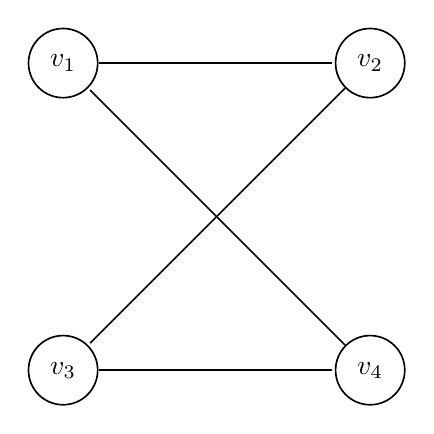
\begin{tikzpicture}[
    > = , % arrow head style
    shorten > = 1pt, % don't touch arrow head to node
    auto,
    node distance = 3cm, % distance between nodes
    semithick % line style
    ]

    \tikzset{every state}=[
    draw = black,
    thick,
    fill = black,
    minimum size = 1mm
    ]

    \node[state] (v1) {$v_1$};
    \node[state] (v2) [right=of v1] {$v_2$};
    \node[state] (v3) [below =of v1] {$v_3$};
    \node[state] (v4) [below =of v2] {$v_4$};
  
    \path[->] (v1) edge  node[]{}(v2);
    \path[->] (v2) edge  node[]{} (v3);
    \path[->] (v3) edge  node[]{}(v4);
    \path[->] (v4) edge  node[]{}(v1);
\end{tikzpicture}\\
{\normalfont{Using definition \ref{adjacent}, 2 adjacent vertices in }}G {\normalfont{are}} $v_1$ {\normalfont{and}} $v_2$. {\normalfont{On the other hand, 2 non adjacent vertices in }}G {\normalfont{are}} $v_1$ {\normalfont{and}} $v_3.$\\
{\normalfont{Using definition \ref{degree}, the degree of every vertex in}} G {\normalfont{is 2}}.
\end{example}
There are many other examples of graphs, one of them being the complete graph on $\mathit{n}$ vertices.
\begin{definition}
\label{Complete Graph}
A graph G(V,E) is said to be complete if $\forall$ v,w $\in$ V v $\neq$ w, v is adjacent to w. The complete graph on n vertices is denoted by $K_n$. \normalfont{\cite{complete_graphs}}
\end{definition}
Given any graph $\mathit{G(V,E)}$, one can also define graph theoretic terminologies that lie within $\mathit{G}$, one of them being a path.
\begin{definition}
\label{Path}
Given a graph G(V,E), a path in G joining any 2 vertices u, v $\in$ V, is a sequence of vertices u = $u_1$, $u_2$, ...,$u_n$ = v in which no vertex is repeated and, $\forall$ 0 $<$  i $<$ n, \{$u_i, u_{i+1}\}$ $\in$ E. {\normalfont{\cite{thompson}}}
\end{definition}
Definition \ref{Path} can now be used to define cycles and connectivity in a graph.
\begin{definition}
\label{connectedgraph}
A graph G(V,E) is said to be connected if $\forall$ u,v $\in$ V u $\neq$ v, u and v are joined by a path. \normalfont{\cite{connected}}
\end{definition}
\begin{definition}
\label{cycle}
Given a graph G(V,E), a cycle in G is a path on n $\geq$ 4 vertices, such that, the first vertex and the last vertex are equal. \normalfont{\cite{cycle}} 
\end{definition}
By definitions \ref{Path}, \ref{cycle} above, it is clear that a cycle is a special instance of a path, with the only difference being that in a cycle, the first vertex and the last vertex are equal. Another thing worth mentioning is that, according to definitions \ref{Path} and \ref{cycle}, cycles and paths are sequences of vertices and not actual graphs. However, this is not the case because they can be represented easily as graphs. For example, given the path/cycle $\mathit{u_1, u_2, ...,u_n}$ a new graph $\mathit{G(V,E)}$ can be created such that, $\mathit{V(G)= \{ u_1, u_2, ..., u_n\}}$ and $\mathit{E(G) = \{ \{u_i, u_{i+1}\} : \forall i, 0 < i < n\}}$. For example, consider the cycle v1 v2 v3 v4 v1, then the graph depicted in example \ref{Example 1}, is the graph representing this cycle. Such graphs are known as Cycle/Path graphs and are denoted by $\mathit{C_n/P_n}$ respecitvely, $\mathit{n}$ being the number of vertices in the graph. Since this construction can be done, cycles/paths will be treated as both graphs and sequences. This will later be useful when defining Hamiltonian cycles. For better understanding of definitions \ref{Complete Graph}, \ref{Path}, \ref{connectedgraph} and \ref{cycle}, example \ref{example3} is constructed.
\begin{example}
\label{example3}
{\normalfont{Consider the graph}} G(V,E) {\normalfont{below:}}\\
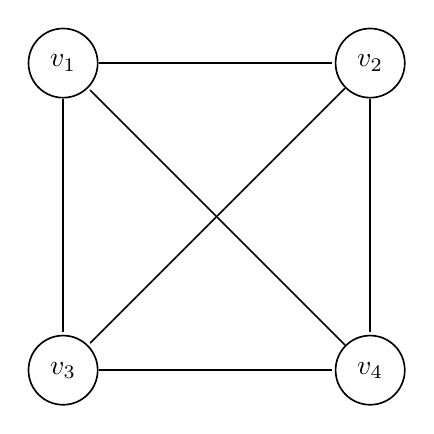
\begin{tikzpicture}[
    > = , % arrow head style
    shorten > = 1pt, % don't touch arrow head to node
    auto,
    node distance = 3cm, % distance between nodes
    semithick % line style
    ]

    \tikzset{every state}=[
    draw = black,
    thick,
    fill = black,
    minimum size = 1mm
    ]

    \node[state] (v1) {$v_1$};
    \node[state] (v2) [right=of v1] {$v_2$};
    \node[state] (v3) [below =of v1] {$v_3$};
    \node[state] (v4) [below =of v2] {$v_4$};
  
    \path[->] (v1) edge  node[]{}(v2);
    \path[->] (v1) edge  node[]{}(v3);
    \path[->] (v2) edge  node[]{} (v3);
    \path[->] (v3) edge  node[]{}(v4);
    \path[->] (v2) edge  node[]{}(v4);
    \path[->] (v4) edge  node[]{}(v1);
\end{tikzpicture}
\\
{\normalfont{Since every vertex in}} G {\normalfont{is adjacent to every other vertex, }}G {\normalfont{must be complete. Therefore}} G {\normalfont{must be}} $K_4$. {\normalfont{Since}} G {\normalfont{is complete, it must also be connected because, there is a path}} $P_2$ {\normalfont{between any 2 distinct vertices of}} G.\\
{\normalfont{Some examples of paths in}} G {\normalfont{are:}}\\
1. $v_1$ $v_2$ $v_3$ $v_4$\\
2. $v_1$ $v_4$\\
3. $v_4$ $v_3$ $v_1$\\
{\normalfont{Some examples of cycles in}} G {\normalfont{are:}}\\
1. $v_1$ $v_2$ $v_3$ $v_4$ $v_1$\\
2. $v_1$ $v_4$ $v_2$ $v_3$ $v_1$\\
3. $v_4$ $v_3$ $v_1$ $v_4$
\end{example}
Another important graph theoretic concept is that of subgraphs. 
\begin{definition}
\label{subgraph}
Given a graph G(V,E) and a graph H($V^\prime$,$E^\prime$), H is a subgraph of G if $V^\prime$ $\subseteq$ V and $E^\prime$ $\subseteq$ E.  \normalfont{\cite{harris_hirst_mossinghoff_2008}}
\end{definition}
After defining some important concepts, the next step is to extend definition \ref{Graph} to define another class of graphs called weighted graphs. It must be noted that all definitions presented so far apply also to weighted graphs.
\begin{definition}
\label{Weighted Function}
Given a graph G(V,E), a weight function is a function f : E $\mapsto$ $\real$ {\normalfont{\cite{harris_hirst_mossinghoff_2008}}}. The real numbers assigned to each edge are called weights.
\end{definition}
\begin{definition}
\label{Weighted Graph}
A weighted graph is a graph G(V,E) with a weight function f {\normalfont{\cite{harris_hirst_mossinghoff_2008}}}. This is denoted by the triple G(V,E,f) or G. 
\end{definition}
According to Bondy and Murty \cite{bondy_murty_1982}, weighted graphs occur regularly in applied graph theory. For example, a railway network can be represented by a weighted graph were, the vertices are the set of towns in the railway network, and there are edges between 2 vertices in the graph if, there is a direct route from one town to another, without visiting other towns in the process. The weight function would then represent the cost of travelling directly from one town to another. In addition to that, the shortest path between 2 towns in the network may be required. It is clear that in order to try and solve such problems, the total weight of a subgraph must first be defined.
\begin{definition}
\label{weightofasubgraph}
Given a weighted graph G(V,E,f), the total weight of any subgraph  H($V^\prime$,$E^\prime$,f) of G is: $$\sum_{e \in E^\prime}^{} f(e) $$. \normalfont{\cite{bondy_murty_1982}}
\end{definition}
It is important to note that by definition \ref{subgraph}, any weighted graph G is a subgraph of itself, therefore, it's weight can be calculated. This is highlighted in Example \ref{example4} below.
\begin{example}
\label{example4}
{\normalfont{Consider the weighted graph}} G(V,E,f) {\normalfont{such that,}} G(V,E) {\normalfont{ is the graph in example \ref{example3} with weight function}} f {\normalfont{such that}},\\
f(\{$v_1, v_2\}$) = 4\\
f(\{$v_1, v_3\}$) = 5\\
f(\{$v_2, v_3\}$) = 2\\
f(\{$v_3, v_4\}$) = 10\\
f(\{$v_2, v_4\}$) = 4\\
f(\{$v_4, v_1\}$) = 7\\
{\normalfont{Then by definition \ref{Weighted Graph}, the graph below is a weighted graph}}.\\
\end{example}
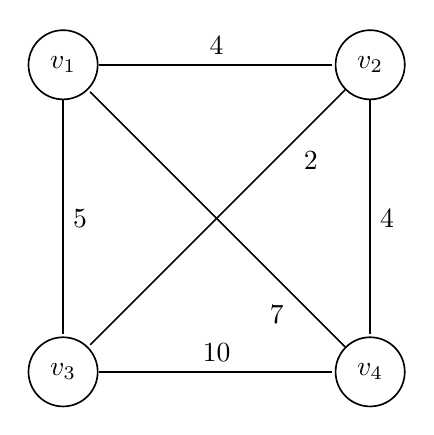
\begin{tikzpicture}[
    > = , % arrow head style
    shorten > = 1pt, % don't touch arrow head to node
    auto,
    node distance = 3cm, % distance between nodes
    semithick % line style
    ]

    \tikzset{every state}=[
    draw = black,
    thick,
    fill = white,
    minimum size = 1mm
    ]
    \node[state] (v1) {$v_1$};
    \node[state] (v2) [right=of v1] {$v_2$};
    \node[state] (v3) [below =of v1] {$v_3$};
    \node[state] (v4) [below =of v2] {$v_4$};
  
    \path[->] (v1) edge  node[]{4}(v2);
    \path[->] (v1) edge  node[]{5}(v3);
    \path[->] (v2) edge  node[pos=0.2,below right]{2} (v3);
    \path[->] (v3) edge  node[]{10}(v4);
    \path[->] (v2) edge  node[]{4}(v4);
    \path[->] (v4) edge  node[pos=0.2,below left]{7}(v1);
\end{tikzpicture}\\
 {\normalfont{Also according to definition \ref{subgraph}, the above graph is a subgraph of itself. Therefore it's weight can be calculated, were by definition \ref{weightofasubgraph}, the weight of}} G {\normalfont{is 32.}}\\
\\
According to Guichard \cite{guichard_2018}, trees are another useful class of graphs.
\begin{definition}
\label{tree}
A tree is a connected graph with no cycles. \normalfont{\cite{guichard_2018}}
\end{definition}
Having defined the basic graph theoretic concepts, it is now time to define harder concepts that use previous definitions. It is important to note that the following concepts can be applied to both weighted and unweighted graphs. Therefore, in the remaining definitions the graph being considered can either be weighted or unweighted.
\begin{definition}
\label{spanning subgraph}
H($V^\prime$,$E^\prime$) is a spanning subgraph of G(V,E) if H is a subgraph of G and $V^\prime$ = V. \normalfont{\cite{ray_2013}}
\end{definition}
There are many spanning subgraphs, however the ones that are relevant to this thesis are spanning trees and spanning cycles, the latter mostly known as Hamiltonian cycles.
\begin{definition}
A graph H is a spanning tree of G if H is a tree and H is a spanning subgraph of G. \normalfont{\cite{ray_2013}}
\label{spanning tree}
\end{definition}
\begin{definition}
\label{hamiltonian cycle}
Given a graph G, c is a Hamiltonian cycle in G if c is a cycle and c is a spanning subgraph of G. Also, a graph that contains a Hamiltonian cycle is called a Hamiltonian graph. \normalfont{\cite{weisstein_2018}}
\end{definition}
It is worth mentioning that definition \ref{hamiltonian cycle} holds because, cycles can be represented by Cycle graphs due to the construction discussed earlier. What follows now is an example that illustrates better definitions \ref{spanning subgraph}, \ref{spanning tree} and \ref{hamiltonian cycle}. 
\begin{example}
\label{example5}
{\normalfont{Let}} G {\normalfont{be the graph in example \ref{example4}. Then, according to definition \ref{spanning subgraph}, the 2 graphs below are 2 spanning subgraphs of}} G {\normalfont{because, they contain all the vertices of}} G {\normalfont{and are subgraphs of }}G .\\
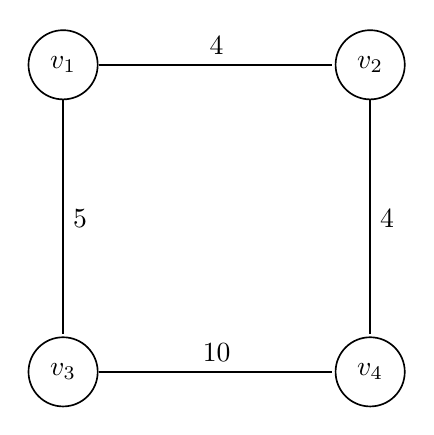
\begin{tikzpicture}[
    > = , % arrow head style
    shorten > = 1pt, % don't touch arrow head to node
    auto,
    node distance = 3cm, % distance between nodes
    semithick % line style
    ]

    \tikzset{every state}=[
    draw = black,
    thick,
    fill = white,
    minimum size = 1mm
    ]
    \node[state] (v1) {$v_1$};
    \node[state] (v2) [right=of v1] {$v_2$};
    \node[state] (v3) [below =of v1] {$v_3$};
    \node[state] (v4) [below =of v2] {$v_4$};
  
    \path[->] (v1) edge  node[]{4}(v2);
    \path[->] (v1) edge  node[]{5}(v3);
    \path[->] (v3) edge  node[]{10}(v4);
    \path[->] (v2) edge  node[]{4}(v4);
\end{tikzpicture}\\
\\
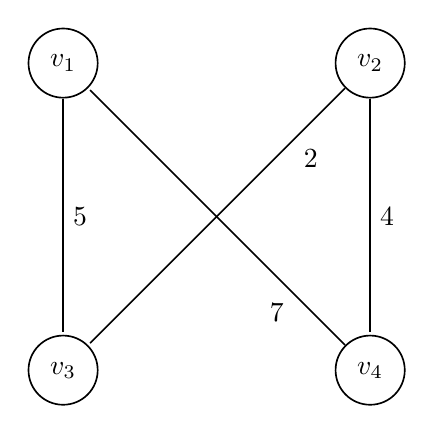
\begin{tikzpicture}[
    > = , % arrow head style
    shorten > = 1pt, % don't touch arrow head to node
    auto,
    node distance = 3cm, % distance between nodes
    semithick % line style
    ]

    \tikzset{every state}=[
    draw = black,
    thick,
    fill = white,
    minimum size = 1mm
    ]
    \node[state] (v1) {$v_1$};
    \node[state] (v2) [right=of v1] {$v_2$};
    \node[state] (v3) [below =of v1] {$v_3$};
    \node[state] (v4) [below =of v2] {$v_4$};
  
    \path[->] (v1) edge  node[]{5}(v3);
    \path[->] (v2) edge  node[pos=0.2,below right]{2} (v3);
    \path[->] (v2) edge  node[]{4}(v4);
    \path[->] (v4) edge  node[pos=0.2,below left]{7}(v1);
\end{tikzpicture}\\
{\normalfont{It must also be said that by definition \ref{hamiltonian cycle}, the above 2 graphs are Hamiltonian cycles in}} G {\normalfont{because, they are spanning subgraphs of}} G {\normalfont{and are Cycle sub-graphs of}} G. {\normalfont{Since the above graphs are subgraphs of }}G{\normalfont{, by definition \ref{weightofasubgraph}, their weight can be calculated by summing up the weights of the edges. Thus, the Hamiltonian cycles above have weight 23 and 18 respectively.}}\\
{\normalfont{Given the same graph }}G{\normalfont{ in example \ref{example4}, the 2 graphs below are spanning trees of }}G{\normalfont{ of weight 18 and 19 respectively.}}\\
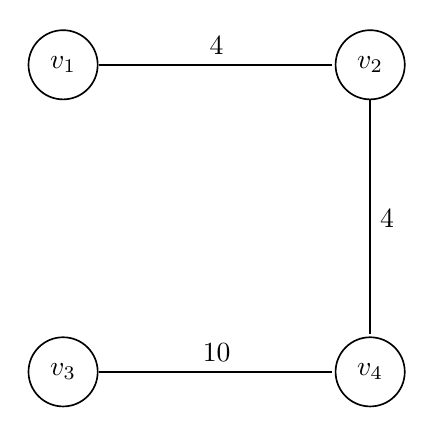
\begin{tikzpicture}[
    > = , % arrow head style
    shorten > = 1pt, % don't touch arrow head to node
    auto,
    node distance = 3cm, % distance between nodes
    semithick % line style
    ]

    \tikzset{every state}=[
    draw = black,
    thick,
    fill = white,
    minimum size = 1mm
    ]
    \node[state] (v1) {$v_1$};
    \node[state] (v2) [right=of v1] {$v_2$};
    \node[state] (v3) [below =of v1] {$v_3$};
    \node[state] (v4) [below =of v2] {$v_4$};
  
    \path[->] (v1) edge  node[]{4}(v2);
    \path[->] (v3) edge  node[]{10}(v4);
    \path[->] (v2) edge  node[]{4}(v4);
\end{tikzpicture}\\
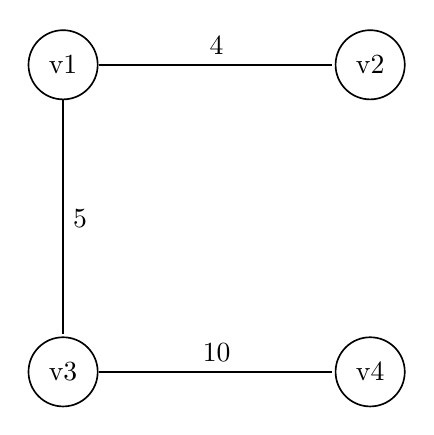
\begin{tikzpicture}[
    > = , % arrow head style
    shorten > = 1pt, % don't touch arrow head to node
    auto,
    node distance = 3cm, % distance between nodes
    semithick % line style
    ]

    \tikzset{every state}=[
    draw = black,
    thick,
    fill = white,
    minimum size = 1mm
    ]
    \node[state] (v1) {v1};
    \node[state] (v2) [right=of v1] {v2};
    \node[state] (v3) [below =of v1] {v3};
    \node[state] (v4) [below =of v2] {v4};
  
    \path[->] (v1) edge  node[]{4}(v2);
    \path[->] (v1) edge  node[]{5}(v3);
    \path[->] (v3) edge  node[]{10}(v4);
\end{tikzpicture}\\
{\normalfont{This example also shows that within the same weighted graph, there could be multiple Hamiltonian cycles and spanning trees of different weight.}}
\end{example}
Having defined Hamiltonian cycles and spanning trees, it is natural to ask whether there are necessary and sufficient conditions in a graph that guarantee it is Hamiltonian or that it contains a spanning tree as subgraph. In fact, theorem \ref{spanningtreetheorem} gives a necessary and sufficient condition for a graph to have a spanning tree.
\begin{theorem}
A graph G has a spanning tree $\iff$ it is connected.
\label{spanningtreetheorem}
\end{theorem} 
\begin{proof}
($\implies$) Let $\mathit{G(V,E)}$ be a graph having a spanning tree $\mathit{T(V^\prime,E^\prime)}$ as one of it's subgraphs. Let $\mathit{v1, v2}$ $\in$ $\mathit{V}$. Since, $\mathit{T}$ is a spanning tree of $\mathit{G}$, then, $\mathit{T}$ is a spanning subgraph of $\mathit{G}$. Thus, $\mathit{v1, v2}$ $\in$ $V^\prime$. Also, since $\mathit{T}$ is a tree, $\mathit{T}$ must be connected. Therefore, $\exists$ a path $\mathit{P}$ joining vertices $\mathit{v_1}$ and $\mathit{v_2}$ in $\mathit{T}$. But since $\mathit{T}$ is a subgraph of G, then $\mathit{P}$ is also a path in $\mathit{G}$. Therefore $\mathit{G}$ must be connected.\\
($\Leftarrow$) Conversely, let $\mathit{G(V,E)}$ be a connected graph. Then, if $\mathit{G}$ has no cycles, $\mathit{G}$ itself must be a spanning tree. If $\mathit{G}$ has cycles, delete an edge from a cycle in $\mathit{G}$. Clearly, the resultant graph is still connected and contains one less cycle. Repeat this procedure untill no more cycles are left in the graph. Then, the resultant graph $\mathit{G^\prime}$ would be a connected subgraph of $\mathit{G}$ having no cycles(i.e a tree). Also, since by the deletion procedure, no vertex was deleted from $\mathit{G}$, $\mathit{G^\prime}$ is a spanning subgraph of $\mathit{G}$. Therefore $\mathit{G^\prime}$ is a spanning tree of $\mathit{G}$. \normalfont{\cite{ray_2013}}
\end{proof}
Theorem \ref{spanningtreetheorem} confirms that for a graph to have a spanning tree, the graph must be connected and vice-versa. Thus, for spanning trees, the necessary and sufficient condition is connectivity. However, the same cannot be said about Hamiltonian cycles because, no necessary and sufficient conditions are known for a graph to be Hamiltonian. In fact, there are sufficient conditions for a graph to be Hamiltonian, however, these conditions are not necessary. According to Guichard \cite{guichard_2018}, these sufficient conditions typically say that for a graph to be Hamiltonian it must have a lot of edges. But it is also argued in \cite{guichard_2018}, that these conditions are not necessary, because, there are Hamiltonian graphs that have few edges. For example, $\mathit{C_n}$ has only $\mathit{n-1}$ edges but is Hamiltonian. One such sufficient but not necessary condition for Hamiltonianicity is Ore's Theorem below.
\begin{theorem}[Ore's Theorem]
\label{ore's theorem}
Let G be a graph on n $\geq$ 3 vertices such that if v and w are not adjacent in G $\implies$ deg(v) + deg(w) $\geq$ n, then G is Hamiltonian.
\end{theorem}
\begin{proof}
Suppose that $\mathit{G(V,E)}$ is a graph satisfying all the conditions in the theorem statement but is not Hamiltonian. Then since $\mathit{G}$ is not Hamiltonian and $K_n$ is Hamiltonian, $\mathit{G}$ must be a subgraph of $\mathit{K_n}$ having fewer edges than $\mathit{K_n}$. Therefore, add edges to $\mathit{G}$ between non adjacent vertices to obtain a subgraph $\mathit{H(V^\prime,E^\prime)}$ of $\mathit{K_n}$ such that adding an edge to $\mathit{H}$ would create a subgraph of $\mathit{K_n}$ which is Hamiltonian. Let $\mathit{u, v}$ $\in$ $V^\prime$ be 2 non-adjecent vertices in H. Since by construction $\mathit{G}$ is a subgraph of $\mathit{H}$, $\mathit{u, v}$ must be non-adjcent in $\mathit{G}$. Therefore $\mathit{deg(u) + deg(v) \geq n}$ in both G and H. Since adding an edge to $\mathit{H}$ creates a resultant graph that is Hamiltonian, then, adding an edge between $\mathit{u}$ and $\mathit{v}$ creates a Hamiltonian graph. Therefore, in $\mathit{H}$ there must be a path joining $\mathit{u}$ and $\mathit{v}$ containing all the vertices of $\mathit{H}$. Let the path be $\mathit{u = v_1, v_2, ..., v_n = v}$.\\
Now suppose $\mathit{deg(v_1)}$ = $\alpha$ in $\mathit{H}$. Now $\forall \mathit{i}, 1 <  i < \mathit{n}$, if there is an edge between $\mathit{u_1}$ and $\mathit{u_i}$ in $\mathit{H}$, then there must not be an edge between $\mathit{u_{i-1}}$ and $\mathit{u_n}$ because, $\mathit{u_1, u_i, u_{i+1}, ..., u_n, u_{i-1}, u_{i-2}, ..., u_1}$ would be a Hamiltonian cycle in $\mathit{H}$, thus H would be Hamiltonian. Therefore, $\mathit{deg(u_n)}$ $\leq$ $\mathit{n-1-\alpha}$\\
$\implies$ $\mathit{deg(u_1) + deg(u_n) \leq \alpha +  n-1 - \alpha}$ in $\mathit{H}$\\
$\implies$ $\mathit{deg(u_1) + deg(u_n) \leq n-1}$ in $\mathit{H}$\\
$\implies$ $\mathit{deg(u_1) + deg(u_n) < n}$ in $\mathit{G}$ since $\mathit{G}$ is a subgraph of $\mathit{H}$.\\
This contradicts the assumption that $\mathit{deg(u_1 = u) + deg(u_n = v) \geq n}$ in $\mathit{G}$ \\
Therefore, $\mathit{G}$ must be Hamiltonian. \cite{ray_2013}
\end{proof}
It is important to note that the above proof uses the fact that $K_n$ is Hamiltonian. This is true because any $C_n$ is always a subgraph of $K_n$. Therefore any $C_n$ that spans $K_n$ is a subgraph of $K_n$. Example \ref{example 6} below is a counter example to show why Ore's theorem gives a sufficient but not necessary condition.\\
\begin{example}
\label{example 6}
{\normalfont{Consider the graph}} $C_5$ below.
\\
\begin{tikzpicture}[
    > = , % arrow head style
    shorten > = 1pt, % don't touch arrow head to node
    auto,
    node distance = 3cm, % distance between nodes
    semithick % line style
    ]

    \tikzset{every state}=[
    draw = black,
    thick,
    fill = white,
    minimum size = 1mm
    ]
    \node[state] (v1) {$v_1$};
    \node[state] (v2) [below left =of v1] {$v_2$};
    \node[state] (v3) [below right =of v1] {$v_3$};
    \node[state] (v4) [below=of v2] {$v_4$};
    \node[state] (v5) [below=of v3] {$v_5$};

    \path[->] (v1) edge  node[]{}(v2);
    \path[->] (v2) edge  node[]{}(v4);
    \path[->] (v4) edge  node[]{}(v5);
    \path[->] (v5) edge  node[]{}(v3);
    \path[->] (v3) edge  node[]{}(v1);
\end{tikzpicture}\\
$C_5$ {\normalfont{above is Hamiltonian because it contains the Hamiltonian cycle}} $v_1, v_2, v_4, v_5, v_3, v_1$. {\normalfont{However,}} deg($v_1$) + deg($v_5$) = 4 $<$ 5 = n. {\normalfont{Therefore, the condition in Ore's Theorem is not a necessary condition}}.
\end{example} 
To conclude, these facts seem to indicate that determining whether a graph is Hamiltonian is a very difficult problem. In addition to that this means that there are certain problems that are harder than other problems. In order to reason about such problems, some computational theory must first be established. This is done in the next subsection.
\subsection{Some Computational Theory}
\newpage
\section{The Travelling Salesman Problem}
\subsection{Heuristics}
\subsection{The Ant Colony Algorithm}
\newpage
\section{Experimental Data}
\newpage
\section{Conclusion}
\newpage
\bibliography{bibliography}
\bibliographystyle{IEEEtran}
\end{document}